
\documentclass[12pt, a4paper]{article}

\usepackage{pdflscape} % pdflscape
\usepackage{graphicx}
\graphicspath{ {./images/} }
%Tarih Ekleme
\usepackage[ddmmyyyy]{datetime}
\renewcommand{\dateseparator}{.}
\renewcommand{\figurename}{Şekil}
\renewcommand{\refname}{Kaynakça}
\usepackage{hyperref}
\usepackage{natbib}

\title{\bf\fontsize{12pt}{14pt}\selectfont KÜTAHYA SAĞLIK BİLİMLERİ ÜNİVERSİTESİ \\ MÜHENDİSLİK VE DOĞA BİLİMLERİ FAKÜLTESİ}
\date{}


\begin{document}
	\maketitle
	
	\begin{center}
		
\includegraphics[width=0.25\linewidth]{ksbu.jpg}
	\end{center}	
	\begin{center}
		\vspace{1cm} 
	\end{center}
	\begin{center}
		\title{\bf\fontsize{12pt}{14pt}\selectfont Latex ile Rapor Hazırlama }
	\end{center}
	\begin{center}
		\vspace{1cm} % Vertical space of 1cm
	\end{center}
	\begin{center}
		
		\author{\bf\fontsize{12pt}{14pt}Halil Şimşek \hspace{1,5cm}2218111004}
		
		\begin{center}
			\vspace{1cm} 
		\end{center}
		\date{\textbf{\today}}
	\end{center}
	\newpage
	
	\section{PostgreSQL Fonksiyonları ve Veri Girişi}
	Proje sürecine uygun olarak bu haftadaki çalışmalarımdan biri PostgreSql'de fonksiyonları öğrenme ve uygulama.
	Database katmanında kitap ekleme ve listeleme işlemini gerçekleştirildi.
	Fonksiyonları öğrenme aşamasında, Murat Yücedağ'ın YouTube kanalından yararlanılmıştır. \cite{kanal:isim}.  \newline
	
	 \begin{figure}[htbp]
		\centering
		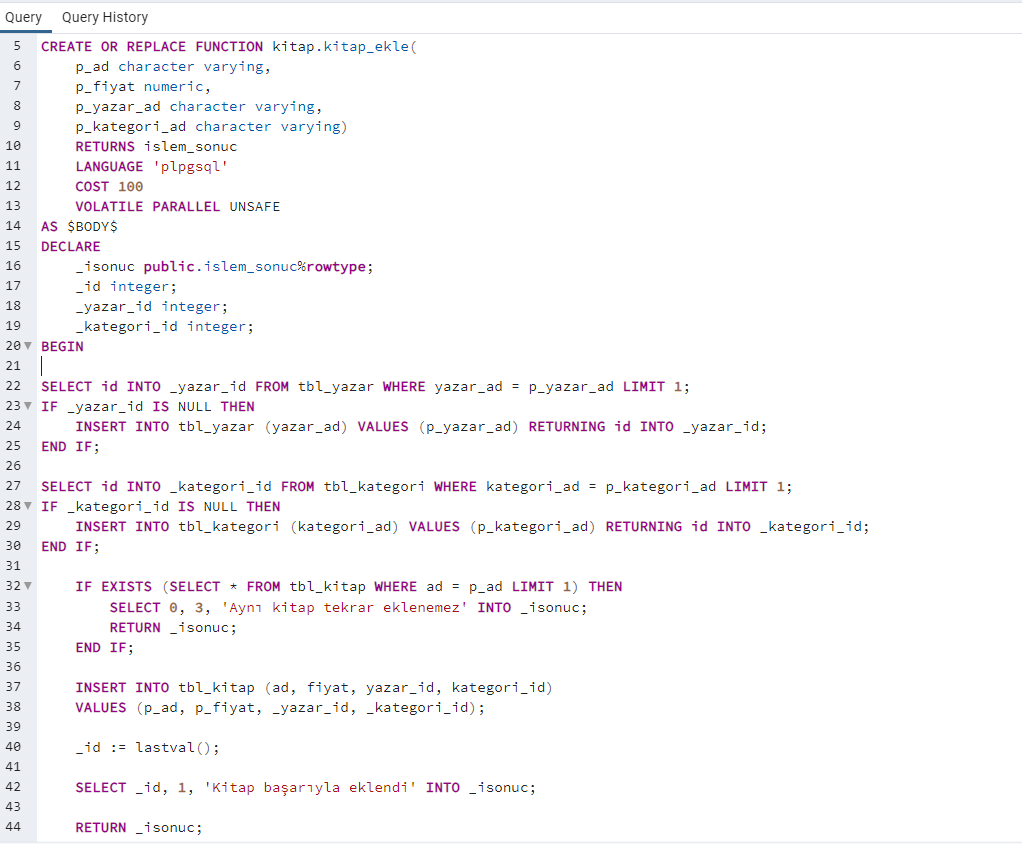
\includegraphics[width=15cm, height=15cm]{ekleFonksiyon.png}
		\caption{PostgreSql'de Fonksiyon Kullanımı}
		\label{fig:fonksiyon}
	\end{figure}

	\subsection{Type Kullanımının Avantajları}
	
	  \begin{figure}[htbp]
		\centering
		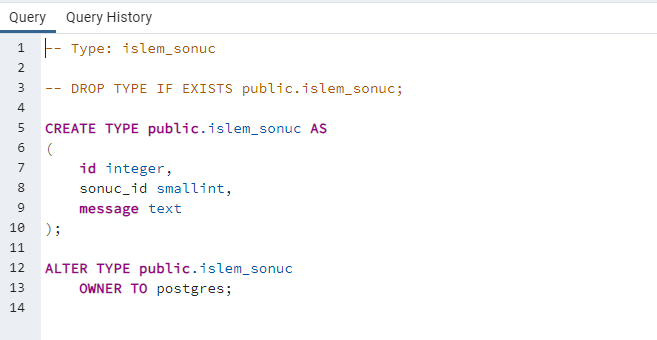
\includegraphics[width=\textwidth, height=8cm]{type.png}
		\caption{Type Kullanımının Gösterimi}
		\label{fig:type}
	\end{figure}
	
	
	\begin{itemize}
		\item Daha İyi Tip Güvenliği: Geri dönüş değeri olarak tip kullanmak, belirli bir türün dönmesini beklediğinizde daha sağlam bir tip güvenliği sağlar. Tip belirtmek, beklenmeyen veri türü dönüşlerine karşı kodunuzu korur ve hataları önler.
		\item Kod Okunabilirliği ve Anlaşılabilirlik: Fonksiyonun geri dönüş değerini belirtmek, kodun daha okunabilir ve anlaşılabilir olmasını sağlar. Fonksiyonun ne tür bir değer döndüreceği hakkında açık bir bilgi verir, bu da kodu anlamayı ve bakımını daha kolay hale getirir.
		\item Dökümantasyon ve API Uyumluluğu: Geri dönüş değerini belirtmek, fonksiyonun dış dünyayla etkileşimini açıklığa kavuşturur. API'ler arasında tutarlılık sağlar ve dış kullanıcılar veya diğer geliştiriciler için fonksiyonun nasıl kullanılacağı hakkında açık bir belge sağlar.
		\item Veri Doğrulama ve Kısıtlamalar: PostgreSQL'de tip kullanarak, geri dönüş değeri üzerinde veri doğrulama ve kısıtlamalar uygulanabilir. Bu, istenmeyen değerlerin dönmesini önler ve veri bütünlüğünü korur.
	\end{itemize}
	
\newpage
	Aynı zamanda ekleme,silme,güncelleme gibi ortak işler için bir type oluşturuldu. Bu type sayesinde yapılan işlemlere göre kullanıcıya bir mesaj verilebilecek.
	Ekleme fonksiyonunu kullanarak veri tabanındaki kitap sayısı da arttrırılmıştır. 
	Type Araştırmasında Chatgpt'den yararlanılmıştır. \cite{chatgpt}
	
	\section{ASP.NET MVC Model Katmanı}

		  \begin{figure}[htbp]
		\centering
		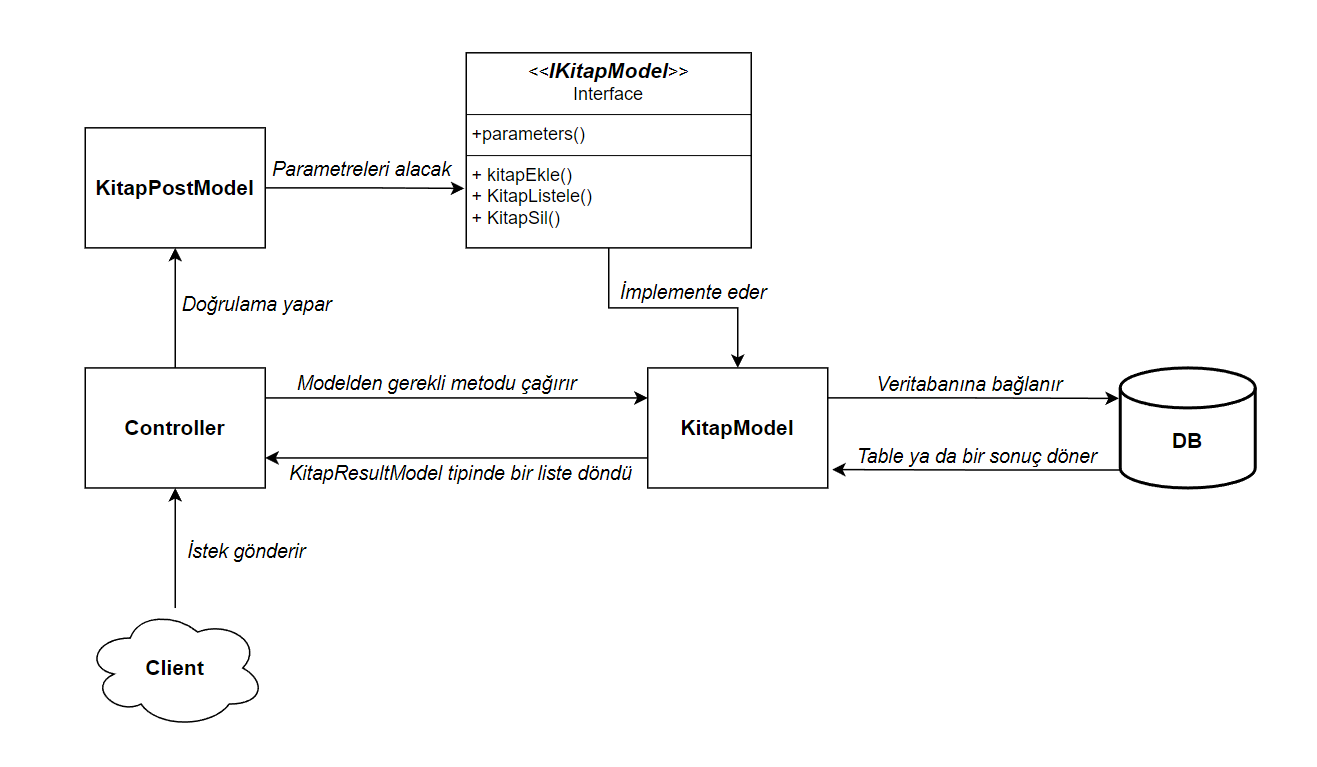
\includegraphics[ width=\textwidth, height=10cm]{mvcSistem.png} 
		\caption{Model Katmanının İşleyişi}
		\label{fig:type}
	\end{figure}
	
	\newpage
	\subsection{IKitapModel Arayüzü}
	Bu arayüz, kitaplarla ilgili işlemlerin sözleşmesini tanımlar. Yani, kitap listeleme ve kitap ekleme gibi işlevlerin prototiplerini içerir.
	KitapListe metodu, kitap listeleme işlemi için gerekli parametreleri (KitapPostModel) alır ve sonuç olarak bir KitapResultModel listesi döndürür. Bu metod, veritabanından kitap listesini almak için kullanılır.
	\newline
	\vspace{8mm}
	
	  \begin{figure}[htbp]
		\centering
		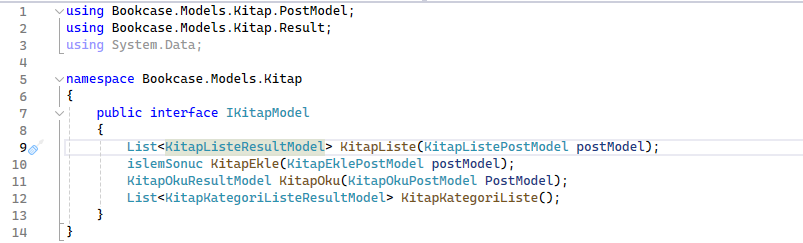
\includegraphics[ width=\textwidth, height=6cm]{IKitapModel.png} 
		\caption{IKitapModel İnterface}
		\label{fig:type}
	\end{figure}
	
	\subsection{KitapModel Sınıfı}
	IKitapModel arayüzünü uygular (implement eder) ve bu arayüzde tanımlanan metodların somut davranışlarını içerir.
	KitapListe metodunun somut uygulaması, PostgreSQL veritabanına bağlanır, bir SQL sorgusu çalıştırır ve sonuçları bir KitapResultModel listesine dönüştürür.Veritabanı bağlantısı ve sorgu işlemleri için NpgsqlConnection ve NpgsqlCommand nesnelerini kullanır.
	\newline
	
	  \begin{figure}[htbp]
		\centering
		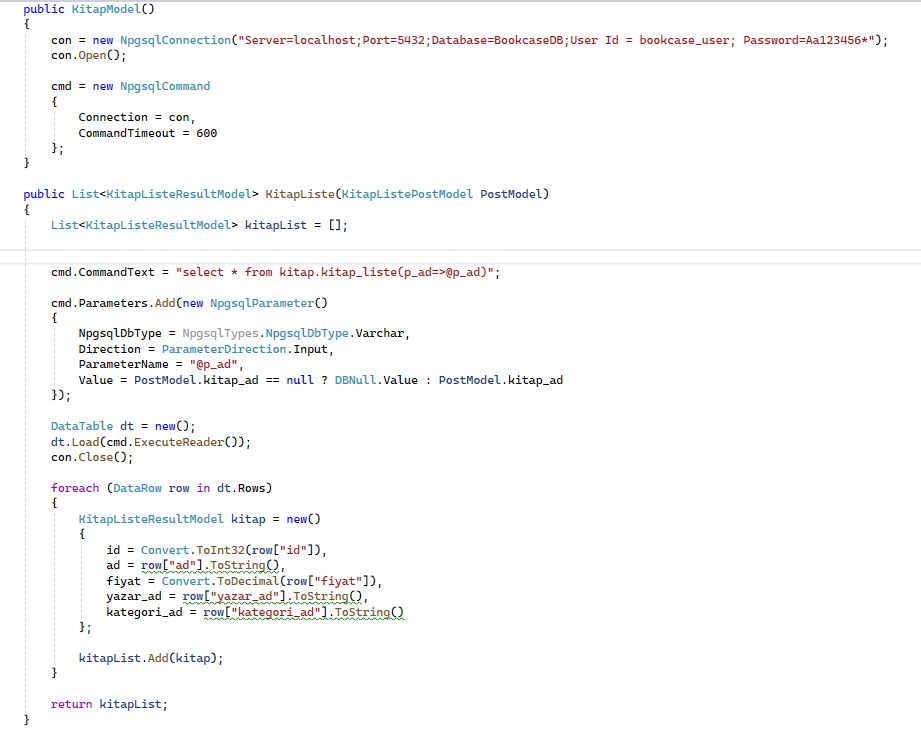
\includegraphics[ width=\textwidth, height=17cm]{KitapModel.png} 
		\caption{KitapModel Sınıfının Kodları}
		\label{fig:type}
	\end{figure}
	\newpage
	
	\subsection{KitapPostModel Sınıfı}	
	Kullanıcıdan alınan verileri taşımak için kullanılır. Bu model, kitap listeleme işlemi sırasında kullanıcı tarafından sağlanan verileri (örneğin, bir kitap adı) içerir.IValidatableObject arayüzünü uygular ve Validate metodu ile modelin kendini doğrulamasını sağlar.Bu arabirim, bir sınıfın Validate metodunu uygulamasını gerektirir.\newline Bu metod, sınıfın kendi doğrulama mantığını içerir ve sınıfın durumunu değerlendirir. Validate metodu, geçerli bir nesne durumunu döndürdüğünde, sınıfın geçerli olduğu anlamına gelir. Geçerli bir nesne durumu döndürülmediğinde ise, sınıfın geçerliliği başarısız olur ve bu durumda hata mesajları veya hata listeleri ile birlikte geçerli olmayan nesne durumu döndürülebilir.
	
	ASP.NET MVC veya ASP.NET Core MVC projelerinde, özellikle model doğrulaması yapmak için sıklıkla IValidatableObject arabirimi kullanılır. Bir modelin belirli doğrulama kurallarını uygulamak ve bu kurallara uygunluğunu kontrol etmek için IValidatableObject arabirimi uygulanabilir. Bu, gelen verilerin doğruluğunu sağlamak için önemli bir mekanizmadır ve hatalı girişlerin önlenmesine yardımcı olur.
	\newline
	\newline
	
		  \begin{figure}[htbp]
		\centering
		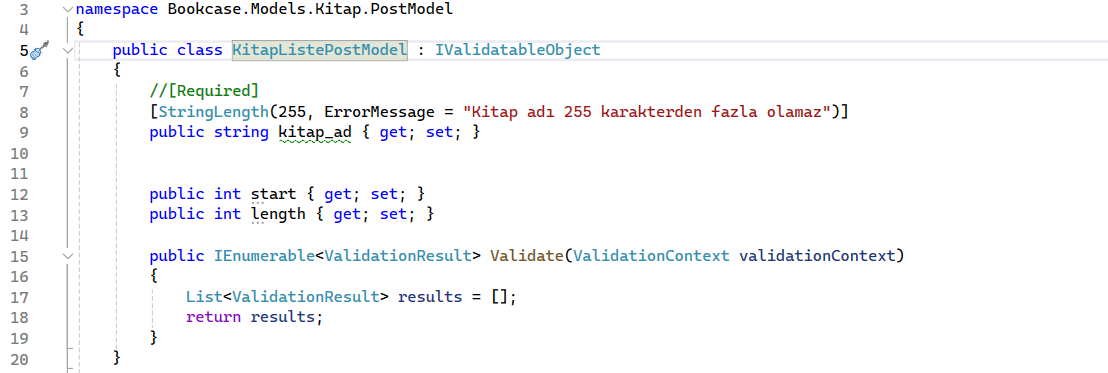
\includegraphics[ width=\textwidth, height=6cm]{KitapPostModel.png} 
		\caption{KitapPostModel Sınıfının Kodları}
		\label{fig:type}
	\end{figure}
	
	\newpage	
	
	\subsection{KitapResultModel Sınıfı}	
	Veritabanından dönen sonuçları temsil eder. Her bir KitapResultModel nesnesi, bir kitap kaydının id, ad, fiyat, yazarAd, kategoriAd gibi özelliklerini içerir.
	\newline \newline
	
		  \begin{figure}[htbp]
		\centering
		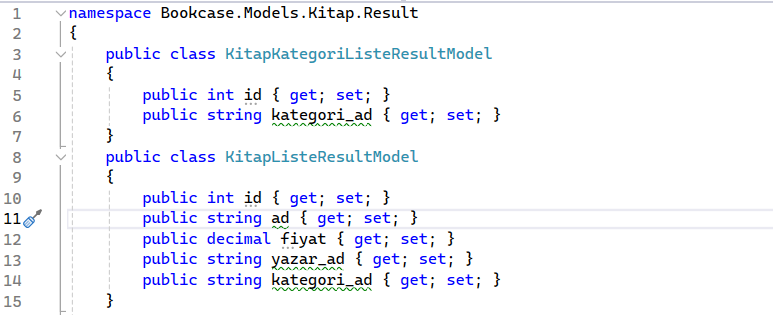
\includegraphics[ width=\textwidth, height=6cm]{KitapResultModel.png} 
		\caption{KitapResultModel Sınıfının Kodları}
		\label{fig:type}
	\end{figure}


	
	\subsection{Controller}	
	MVC'nin Controller bileşenidir ve kullanıcı isteklerini yönetir.
	Index metodu, uygulamanın ana sayfasını döndürür ve genellikle kullanıcıya HTML içeriği sunar.
	kitapListe metodu, bir HTTP POST isteği ile çağrıldığında, KitapListePostModel tipindeki veriyi alır, modelin geçerliliğini kontrol eder ve KitapModel üzerinden kitap listesini çeker. Daha sonra bu listeyi JSON formatında istemciye (web tarayıcısına) geri döndürür.
\newpage
			  \begin{figure}[htbp]
		\centering
		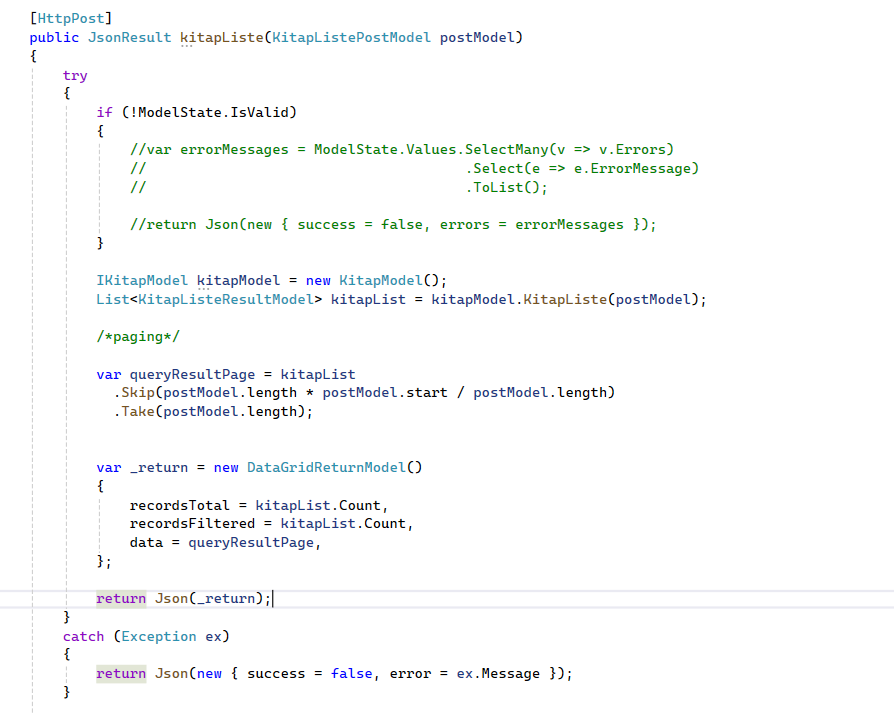
\includegraphics[ width=\textwidth, height=15cm]{Controller.png} 
		\caption{Controller Sınıfının Kodları}
		\label{fig:type}
	\end{figure}
\newpage

\section{Listeleme İşleminin Gerçekleştirilmesi}
	
	Listeleme işlemi yapılırken hazır grid kullanılmıştır. Grid bu websiteden alınmıştır. \cite{datatables}. Bootstrap kütüphanesinden yararlanılmıştır. Bootstrap hakkındaki araştırmalar ve öğrenimler de \cite{bootstrap} sitesinden yararlanılmıştır. Listelenen gridin son hali şekil:9 da bulunmaktadır.
	

		  \begin{figure}[htbp]
		\centering
		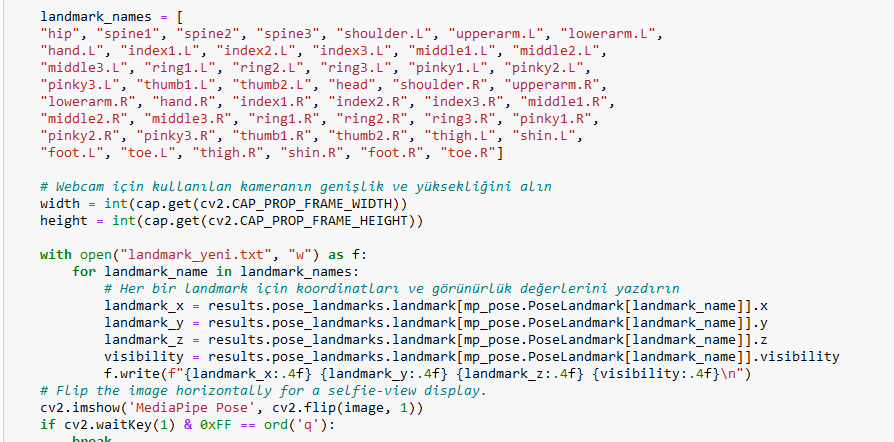
\includegraphics[ width=\textwidth, height=11cm]{liste.png} 
		\caption{Listelenen Veriler}
		\label{fig:type}
	\end{figure}
	
		\newpage
	\begin{thebibliography}{9}
		\bibitem{kanal:isim}
		Murat Yücedağ, "Murat Yücedağ YouTube Kanalı", YouTube. \url{https://www.youtube.com/MurattYucedag}
		\bibitem{chatgpt} ChatGPT, OpenAI. \url{https://openai.com/gpt}
		
		
	\end{thebibliography}
	
	%Kaynakçayı yazdırmak
	
	%\printbibliography %Prints bibliography
	
	
\end{document}